\documentclass{article}

\usepackage[numbers, compress]{natbib}

\usepackage[utf8]{inputenc} % allow utf-8 input
\usepackage[T1]{fontenc}    % use 8-bit T1 fonts
\usepackage{hyperref}       % hyperlinks
\usepackage{url}            % simple URL typesetting
\usepackage{booktabs}       % professional-quality tables
\usepackage{amsfonts}       % blackboard math symbols
\usepackage{nicefrac}       % compact symbols for 1/2, etc.
\usepackage{microtype}      % microtypography

\usepackage{amsthm,amsmath,amssymb}
\usepackage{macros}
\usepackage{subcaption}
\usepackage[textfont=small, labelfont=small]{caption}
\usepackage{graphicx}
\DeclareGraphicsExtensions{.pdf,.png,.jpg,.eps}

\usepackage{algorithm}
\usepackage{algorithmic}

\usepackage[color=yellow]{todonotes}
\usepackage{booktabs}
\usepackage[inline]{enumitem}
\usepackage{verbatim}

\usepackage[left=1.5in, right=1.5in, top=1.25in, bottom=1.25in]{geometry}

\usepackage{setspace}


\title{Discrete and continuous latent states of neural activity in \textit{Caenorhabditis Elegans}}

\author{Scott W. Linderman 
  and
  Liam Paninski \\
  Columbia University
}


\begin{document}

\singlespacing
\maketitle

\begin{abstract}
  Recent advances in neural recording technologies have enabled
  simultaneous measurements of the majority of head ganglia neurons in
  immobilized C. elegans \cite{kato2015global}. Moreover, since some
  neurons are known to reliably indicate the onset or offset of
  particular behaviors, like ventral and dorsal turns, behavioral
  state can be decoded from the simultaneous population recordings.
  These datasets provide unique visibility into the relationship
  between neural activity and behavior.  While it seems clear that
  activity is inherently lower dimensional than the number of neurons
  due to strong correlations between cells, the nature of the latent brain state
  remains unclear. For example, is brain state better thought of as
  discrete or continuous, or perhaps a combination of the two? Does it
  obey linear or nonlinear dynamics?  We propose a generative approach
  to probing these questions. We model the neural activity as a
  \emph{switching linear dynamical system} (SLDS), with both discrete
  and continuous latent states, and conditionally linear dynamics.  We
  then analyze the posterior distribution over states implied by the
  neural recordings and find that the discrete states correspond to
  stereotypical motor sequences. In contrast to previous work, these
  states are exposed in an entirely unsupervised manner.
\end{abstract}

% Body
\onehalfspacing

\section{Model}

\begin{figure}[t]
\centering%
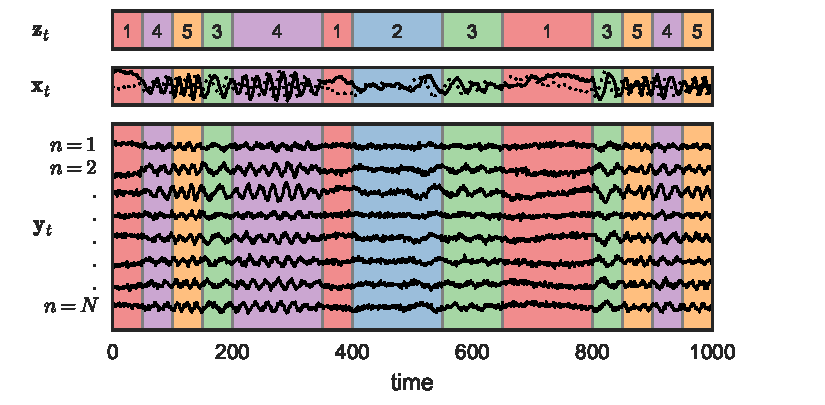
\includegraphics[width=5.5in]{slds} 
\caption{Simulated data from a switching linear dynamical system.
The population stochastically jumps between discrete states,~$z_t \in \{a,b,c,d\}$,
each of which is color coded for visualization.
These discrete states govern the linear dynamics of the continuous latent 
state,~$\bx_t \in \reals^D$ (here,~$D=2$). For example, state~$a$ corresponds to a simple
random walk, whereas state~$d$ has fast, oscillatory dynamics. Finally,
the observed signals,~$\by_t \in \reals^N$ (here,~$N=8$), are obtained via a linear 
transformation of the underlying, continuous state,~$\bx_t$. The correlations
and dynamics in the observations are inherited from the dynamics of the
latent states.}
\vspace{-0.5cm}
\label{fig:slds_ex}
\end{figure}

Assume the instantaneous neural activity at time~$t$ for a population
of~$N$ neurons is represented as a vector,~$\by_t \in \reals^N$. In
calcium imaging settings, the entries in this vector may be
instaneous~$\Delta F/F$ measurements, or another signal that captures
neural activity. In this experiment, we use the smoothed time
derivative of~$\Delta F/F$. Over the course of an experiment, we
measure a sequence of vectors, which we combine into a matrix denoted
by~$\by_{1:T}$.

Our model is based on the following assumptions: (i) the instantaneous
neural activity,~$\by_t$, reflects an underlying, low-dimensional
latent state; (ii) this state has a discrete component,~$z_t \in \{1, \ldots, K\}$,
and a continuous component,~$\bx_t \in \reals^D$; (iii) the continuous
latent state has linear dynamics governed by the corresponding discrete
latent state; and (iv) the observed neural activity is a linear function
of the underlying states with additive Gaussian noise.  

\TODO{Discuss the motivation for these modeling assumptions.}

These assumptions
are combined in a switching linear dynamical system, which we formalize 
with the following generative model:
\begin{align}
  \label{eq:joint}
  p(\by_{1:T}, \bx_{1:T}, \bz_{1:T} \given \bTheta) &= 
  p(\bTheta)
  \prod_{t=1}^T
  p(z_t \given z_{t-1}, \bTheta) \, 
  p(\bx_t \given z_{t-1}, \bx_{t-1}, \bTheta) \, 
  p(\by_t \given z_t, \bx_t, \bTheta).
\end{align}
Our beliefs about the dynamics of these latent states are encoded in the 
form of the conditional distributions for~$z_t$ and~$\bx_t$. First,
we assume the discrete states follow a Markov process,
\begin{align}
  p(z_t \given z_{t-1}, \bTheta) &\sim \distDiscrete(\bpi^{(z_{t-1})}).
\end{align}
Next, we imbue the continuous latent states with linear Gaussian dynamics,
\begin{align}
  p(\bx_t \given \bx_{t-1}, z_{t-1}, \bTheta) 
  &\sim \distNormal(\bA^{(z_{t-1})} \bx_{t-1} + \bb^{(z_{t-1})}, \bQ^{(z_{t-1})}).
\end{align}

% Figure illustrating latent dynamics
\begin{figure}[t]
\centering%
\begin{subfigure}{.49\textwidth}
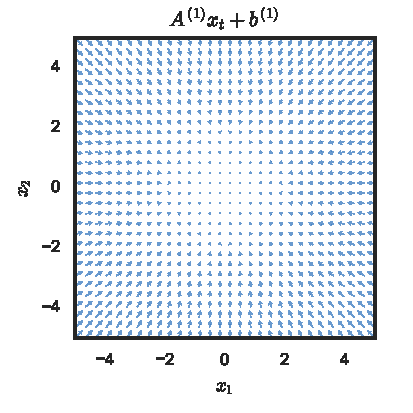
\includegraphics[width=\textwidth]{dynamics_1}
\end{subfigure} 
\begin{subfigure}{.49\textwidth}
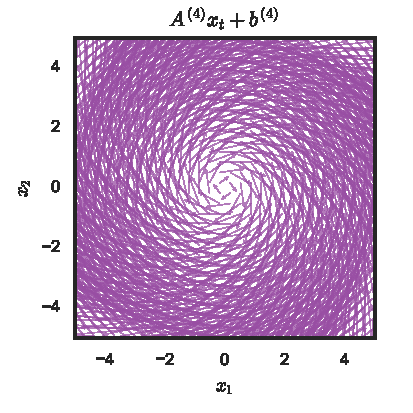
\includegraphics[width=\textwidth]{dynamics_4}
\end{subfigure} 
\caption{The dynamics corresponding to discrete latent state~$k$ may
  be visualized as a vector field where the arrows point to the
  expected next state,~$\bbE[\bx_{t+1}]=\bA^{(k)}\bx_t + \bb^{(k)}$.
Here, we show the dynamics for the first and fourth discrete states 
in the synthetic example from Figure~\ref{fig:slds_ex}. The first 
discrete state is a random walk with a slight decay toward the origin;
the fourth discrete state corresponds to fast, oscillatory dynamics.}
\label{fig:slds_dynamics_ex}
\vspace{-0.5cm}
\end{figure}



Finally, we impose the assumption of linear observations via the conditional
distribution,
\begin{align}
  p(\by_t \given \bx_{t}, z_{t}, \bTheta) 
  &\sim \distNormal(\bC^{(z_{t})} \bx_{t} + \bd^{(z_{t})}, \bR^{(z_t)}).
\end{align}
Thus, the parameters of the model are,
\begin{align}
  \bTheta &= \left\{ \bA^{(k)}, \bb^{(k)}, \bQ^{(k)}, \bC^{(k)}, \bd^{(k)}, \bR^{(k)}, \bpi^{(k)} \right\}_{k=1}^K .
\end{align}

\TODO{Discuss interpretation of the parameters. Set the stage for visualizing~$\bA^{(k)}$ 
in later sections.}


\section{Results}

\bibliographystyle{unsrt}
\bibliography{writeup}

\appendix

\section{Bayesian Inference for Switching Linear Dynamical Systems}
Our goal is to estimate the posterior probability of a sequence 
of latent states and a set of parameters given the observed data.
From Bayes' rule, we have,
\begin{align}
  p(\bz_{1:T}, \bx_{1:T}, \bTheta \given \by_{1:T}) 
  &= 
  \frac{p(\by_{1:T}, \bx_{1:T}, \bz_{1:T}, \bTheta)}{p(\by_{1:T})}.
\end{align}
The numerator is the joint probability given by Eq.~\eqref{eq:joint}, and
the denominator,~$p(\by_{1:T})$, which is also known as the
\emph{marginal likelihood}, is given by an integral over possible
latent states and parameters,
\begin{align}
  p(\by_{1:T}) &= \int p(\by_{1:T}, \bx_{1:T}, \bz_{1:T}, \bTheta) 
  \, \mathrm{d}\bx_{1:T} \, \mathrm{d}\bz_{1:T} \, \mathrm{d}\bTheta.
\end{align}
Unfortunately, this integral is not efficiently computable for complex
models like the SLDS, forcing us to seek approximate inference methods
instead. Markov chain Monte Carlo (MCMC) methods \todo{cite} offer one
such approach. 

To construct our MCMC algorithm, we iteratively sample one set of 
latent states or parameters from its conditional distribution, holding 
the rest fixed, in a technique known as Gibbs sampling \todo{cite}. 
There are five main sets of parameters to sample, detailed below.
\begin{enumerate}
  \item \textit{Gibbs sampling the discrete latent states,~$\bz_{1:T}$:}
    
    Given the continuous latent states,~$\bx_{1:T}$, and the
    parameters,~$\bTheta$, the conditional distribution over discrete
    latent states is the same as in a standard hidden Markov model. A
    joint sample from~$p(\bz_{1:T} \given \bx_{1:T}, \by_{1:T},
    \bTheta)$ can be generated using the forward filtering backward
    sampling (FFBS) algorithm.

  \item \textit{Gibbs sampling the continuous latent states,~$\bx_{1:T}$:}
    
    Given the discrete latent states,~$\bz_{1:T}$, the observations,~$\by_{1:T}$,
    and the parameters,~$\bTheta$, the conditional distribution of the 
    continuous latent states is linear and Gaussian. As with the discrete
    latent states, a joint sample of~$p(\bx_{1:T} \given \bz_{1:T}, \by_{1:T}, \bTheta)$
    can be generated using an FFBS algorithm.

  \item \textit{Gibbs sampling the dynamics parameters,~$\{\bA^{(k)}, \bb^{(k)}, \bQ^{(k)}\}_{k=1}^K$:}
    
    For fixed latent state sequences, the dynamics model reduces to a simple 
    multivariate regression problem. We have,
    \begin{multline}
      p(\bA^{(k)}, \bb^{(k)}, \bQ^{(k)}  \given \bz_{1:T}, \bx_{1:T}, \by_{1:T}, \bTheta)
      \\ 
      \propto
      p(\bA^{(k)}, \bb^{(k)}, \bQ^{(k)})
      \prod_{t=1}^T \left[ \,
        \distNormal(\bx_{t} \given \bA^{(k)} \bx_{t-1} + \bb^{(k)},\, \bQ^{(k)} \right]^{\bbI[z_{t-1}=k]}.
    \end{multline}
    If the prior distribution is the form of a matrix normal inverse Wishart (MNIW) prior, 
    then this conditional distribution will be as well. 

  \item \textit{Gibbs sampling the observation parameters,~$\{\bC^{(k)}, \bd^{(k)}, \bR^{(k)}\}_{k=1}^K$:}
    
    As with the dynamics parameters, 
    for fixed latent state sequences, the observation model is also a 
    multivariate regression problem. We have,
    \begin{multline}
      p(\bC^{(k)}, \bd^{(k)}, \bR^{(k)}  \given \bz_{1:T}, \bx_{1:T}, \by_{1:T}, \bTheta)
      \\ 
      \propto
      p(\bC^{(k)}, \bd^{(k)}, \bR^{(k)})
      \prod_{t=1}^T \left[ \,
        \distNormal(\by_{t} \given \bC^{(k)} \bx_{t} + \bd^{(k)},\, \bR^{(k)} \right]^{\bbI[z_{t}=k]}.
    \end{multline}
    This, too, is conjugate when the prior distribution assumes the
    form of a matrix normal inverse Wishart (MNIW) distribution.

  \item \textit{Gibbs sampling the Markov parameters,~$\{\bpi^{(k)}\}_{k=1}^K$:}
    
    Finally, we must sample the Markov transition matrix. We separate
    this into its~$K$ rows, each of which specifies a probability
    distribution,~$p(z_t \given z_{t-1}=k) = \bpi^{(k)}$.  For a fixed
    discrete latent state sequence, the conditional distribution of~$\bpi^{(k)}$ 
    is,
    \begin{align}
      p(\bpi^{(k)} \given \bz_{1:T}) &\propto
      p(\bpi^{(k)}) \prod_{t=1}^T \left[ \pi_{z_t}^{(k)} \right]^{\bbI[z_{t-1}=k]}.
    \end{align}
    If the prior distribution is~$p(\bpi^{(k)}) = \distDirichlet(\bpi^{(k)} \given \alpha)$, then this
    conditional distribution is a Dirichlet as well,
    \begin{align}
      p(\bpi^{(k)} \given \bz_{1:T}) 
      &= \distDirichlet(\bpi^{(k)} \given \widetilde{\balpha}^{(k)}) \\
      \widetilde{\alpha}_{k'}^{(k)} &= \alpha + \sum_{t=1}^T \bbI[z_t = k'] \, \bbI[z_{t-1}=k].
    \end{align}
\end{enumerate} 

Each one of these five steps leaves the desired posterior distribution as the 
unique stationary distribution of the Markov chain. Thus, by iterating these 
steps, the sampled states and parameters will eventually be distributed according
to their posterior probability given the observed data. Critically, the rate 
at which the Markov chain converges to its stationary distribution is determined
in part by the correlation between the sampled latent states at one iteration and
those at the next. If the chain only makes minor updates to the latent state sequence,
it will likely take a long time to converge to the desired posterior distribution.  
By performing joint, ``block'' updates of~$\bx_{1:T}$ and~$\bz_{1:T}$ in steps 
1 and 2, we find that the latent state sequences are able to be explored more 
efficiently.

\end{document}
